
%(BEGIN_QUESTION)
% Copyright 2011, Tony R. Kuphaldt, released under the Creative Commons Attribution License (v 1.0)
% This means you may do almost anything with this work of mine, so long as you give me proper credit

One of the major processes used to treat municipal wastewater is {\it aeration}, where the dissolved oxygen concentration of the wastewater is enhanced by bubbling air through the water in an {\it aeration basin}.  A dissolved oxygen (``DO'') analyzer measures the oxygen concentration in the wastewater, and a controller varies the speeds of blowers pumping air into the basins using AC motors powered through variable-frequency drives (VFDs):

$$\includegraphics[width=15.5cm]{i03292x01.eps}$$

A problem with this particular system is that the nozzles at the bottom of the aeration chamber have a tendency to plug up, thus impeding air flow into the chamber.  The controller (AIC) will compensate for this over time by commanding the blowers to spin faster, but the correction is not immediate which results in temporary deviations from setpoint. 

\vskip 10pt

Modify this control strategy so that any plugging of the nozzles will be immediately sensed and compensated for, avoiding the temporary deviations from setpoint.  Feel free to add any needed field instruments to make this happen.

\vfil 

\underbar{file i03292}
\eject
%(END_QUESTION)





%(BEGIN_ANSWER)

This is a graded question -- no answers or hints given!

%(END_ANSWER)





%(BEGIN_NOTES)

The basic problem we face here is one of a {\it load change} affecting process stability, the load in this case being plugging of the air nozzles.  Since the offending load happens to exist on the very same line that our final control element (each VFD-powered blower) resides on, the best strategy for compensation is {\it cascade} whereby we make the affected variable stable with a slave control loop:

$$\includegraphics[width=15.5cm]{i03292x02.eps}$$

Since each set of distribution nozzles is liable to independently plug, it is best to have two cascaded flow control loops (one per nozzle array) slaved off the same master analytical controller.

\vskip 10pt

It would be a mistake to try to apply feedforward control to this problem, since the load in this case is something we can definitely control.  Feedforward is best suited for loads which we have no control over (i.e. ``wild'' variables), and where the compensation takes place on a different variable.  Cascade is best suited for loads we can force to become stable using the existing final control element.

%INDEX% Control, strategies: cascade
%INDEX% Process: wastewater aeration (dissolved oxygen control)

%(END_NOTES)


